\documentclass{beamer}
 
\usepackage{listings}
\usepackage[utf8]{inputenc}

 \lstdefinestyle{customc}{
  belowcaptionskip=1\baselineskip,
  breaklines=true,
  frame=L,
  xleftmargin=\parindent,
  language=C,
  showstringspaces=false,
  keywordstyle=\bfseries\color{green!40!black},
  commentstyle=\itshape\color{purple!40!black},
  identifierstyle=\color{blue},
  stringstyle=\color{orange},
}

\lstset{escapechar=@,style=customc,numbers=left,literate={~} {$\sim$}{1}}


%TODO
% add Frederic
% add frame number
% table of contents
 
%Information to be included in the title page:
\title{Software Fault Isolation using the CompCert compiler}
\author{Alexandre Dang}
\institute{Team Celtique}
 
\begin{document}
\frame{\titlepage}
 

%%%%%%%%%%%%%%%%%%%%  SFI  %%%%%%%%%%%%%%%%%%%%
\section{Software Fault Isolation}
\label{sec:Software Fault Isolation}

\begin{frame}[c]{Flash sux}
\end{frame}

\begin{frame}{Goals of Software Fault Isolation (SFI)}
	\begin{itemize}
		\item SFI aims to allow a protected program to execute dangerous modules in its own memory space without dangers. 
		\item SFI confines the execution of the dangerous modules in a reserved area called sandbox
		\item \texttt{jump} and \texttt{write} instructions are protected by runtime checks
		\item function calls to the protected programs are controlled by SFI
	\end{itemize}
\end{frame}

\begin{frame}[c]{Goals of SFI}
\begin{figure}
\centering
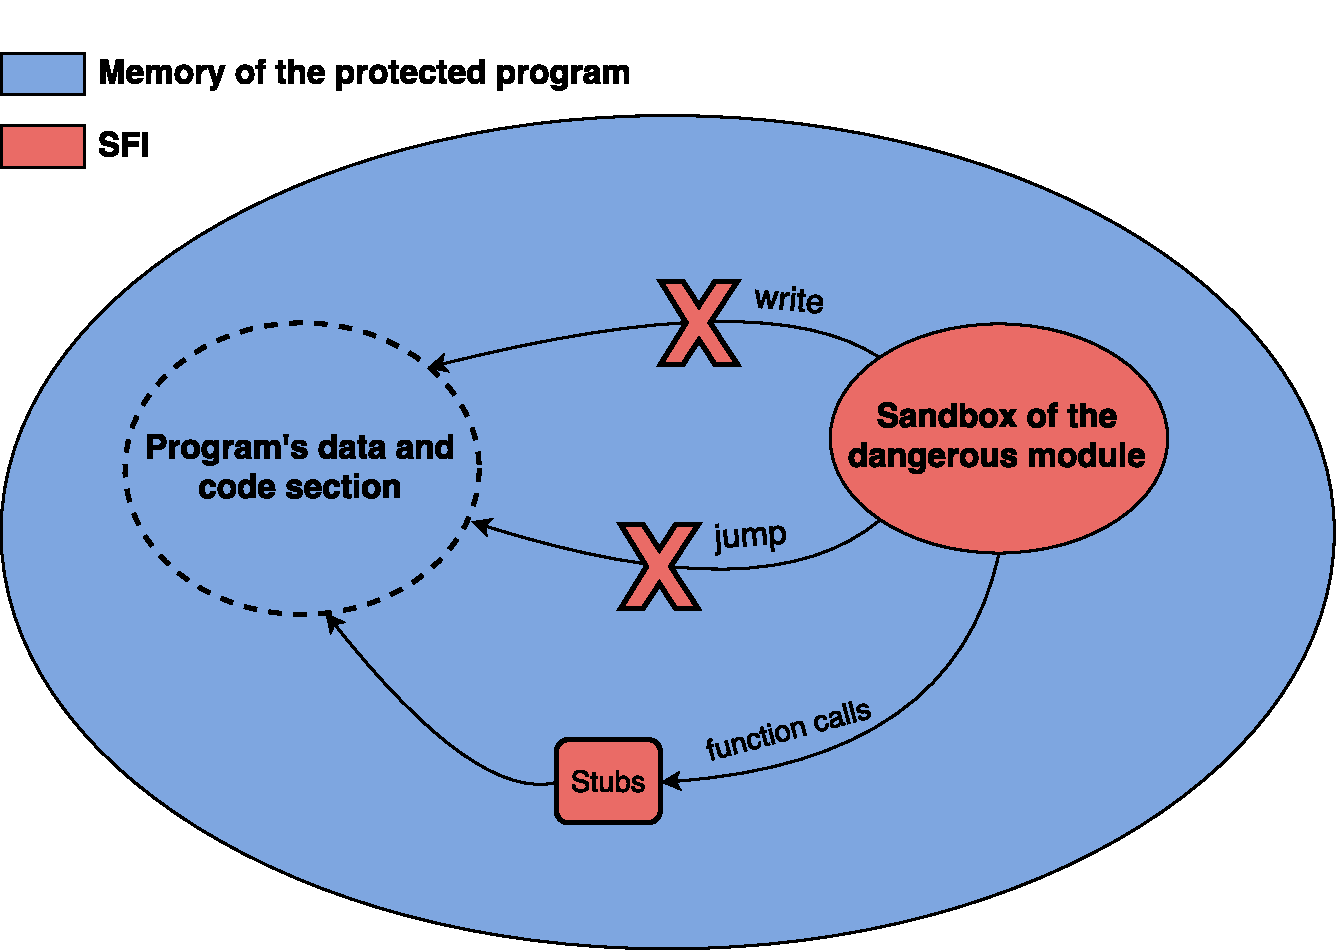
\includegraphics[width=1\textwidth]{images/sfi_principle.pdf}
\end{figure}

\end{frame}

\begin{frame}{Overview of SFI} %code gen + verifier
	SFI chain is composed of two elements: a generator and a verifier
		\begin{itemize}
			\item the generator transforms the assembly code of the dangerous modules in order to confine the modules in their sandbox
			\item the verifier checks that the SFI transformations are present and valid before loading the code in memory
		\end{itemize}
\end{frame}

\begin{frame}{Sandboxing}
	Sandbox are continuous area identified by a tag
	For example the sandbox [\texttt{0xda000000}~-~\texttt{0xdaffffff}] has the tag \textbf{\texttt{0xda}}
\end{frame}

\begin{frame}[c]{NativeClient}
	Google im
\end{frame}

\begin{frame}[c]{SFI for CompCert}
\end{frame}

\begin{frame}{Advantages of SFI}
\end{frame}

\begin{frame}[c]{Problematics of SFI}
\end{frame}

%%%%%%%%%%%%%%%%%%%%  ROP  %%%%%%%%%%%%%%%%%%%%
\section{Return Oriented Programing attacks}
\label{sec:Return Oriented Programing attacks}

\begin{frame}[c]{Return Oriented Programing attacks}
\end{frame}

\begin{frame}[fragile]{Example (1/2)}
\begin{lstlisting}
	void evil_code() {
		printf("Argh, we got hacked!\n");
	}

	void foo(char* input){
		char buf[1];
		... code ...
		strcpy(buf, input);
		... code ...
	}
\end{lstlisting}

\end{frame}

\begin{frame}[fragile]{Example (2/2)}
\textcolor{gray}{terminal\$~} ./buffer \$(python -c 'print 13*"a"+"\textbackslash{x7b}\textbackslash{x84}\textbackslash{x04}\textbackslash{x08}"') \\
\textcolor{red}{Address of evil\_code = 0x0804847b} \\
Stack before: \hfill \break
0xf7712000    \hfill \break
0xff957998    \hfill \break
0xf7593d26    \hfill \break
0xf7712d60    \hfill \break
0x0804868c    \hfill \break
0xff957978    \hfill \break
0xf7593d00    \hfill \break
0xf7713dc0    \hfill \break
0xf77828f8    \hfill \break
0xff957998    \hfill \break
0x08048510    ~~~~~~~~~~~~~~~~\textcolor{blue}{//Return address of \textit{foo}}\hfill \break
              \hfill \break
Stack after : \hfill \break
0xff958161    \hfill \break
0xff957998    \hfill \break
0xf7593d26    \hfill \break
0xf7712d60    \hfill \break
0x0804868c    \hfill \break
0xff957978   			   ~~~~~~~~~~~~~~~~\textcolor{blue}{//Buffer overflow}\hfill \break
\textcolor{red}{0x61}593d00~~~~~~~~~~~~~~~~\textcolor{blue}{//``a''   } \hfill \break
\textcolor{red}{0x61616161}~~~~~~~~~~~~~~~~\textcolor{blue}{//``aaaa''} \hfill \break
\textcolor{red}{0x61616161}~~~~~~~~~~~~~~~~\textcolor{blue}{//``aaaa''} \hfill \break
\textcolor{red}{0x61616161}~~~~~~~~~~~~~~~~\textcolor{blue}{//``aaaa''} \hfill \break
\textcolor{red}{0x0804847b}~~~~~~~~~~~~~~~~\textcolor{blue}{//"\textbackslash{x7b}\textbackslash{x84}\textbackslash{x04}\textbackslash{x08}",  \textit{evil\_code} address \\}
\\
Argh, we got hacked! ~~\textcolor{blue}{//Success! \textit{evil\_code} was executed}\\
Segmentation fault (core dumped)

\end{frame}
\begin{frame}[c]{Modern ROP attacks}
\end{frame}

%%%%%%%%%%%%%%%%%%%%  Overview  %%%%%%%%%%%%%%%%%%%%
\section{Overview of our approach}
\label{sec:Overview of our approach}

\begin{frame}[c]{Goals of our approach}
\end{frame}

\begin{frame}[c]{CompCert stack}
\end{frame}

\begin{frame}[c]{Transformations of the stack layout}
\end{frame}

\begin{frame}[c]{Injection of runtime checks}
\end{frame}

\begin{frame}[c]{Conditions of our approach}
\end{frame}

\begin{frame}[c]{Discussion of the approach}
\end{frame}

%%%%%%%%%%%%%%%%%%%%  Evaluation  %%%%%%%%%%%%%%%%%%%%
\section{Evaluation}
\label{sec:Implementation}

\begin{frame}[c]{Evaluation of security}
\end{frame}

\begin{frame}[c]{Evaluation of performance}
\end{frame}

\begin{frame}[c]{Discussion}
\end{frame}

 
\end{document}


